\section{Quadtrees}
\subsection{Introduction}
\begin{frame}
    \frametitle{Quadtrees}
    Divide some given space according to its \emph{particle density}
    \begin{figure}
        \centering
        \resizebox{\textwidth}{!}{%
            \section{Quadtrees}
\subsection{Introduction}
\begin{frame}
    \frametitle{Quadtrees}
    Divide some given space according to its \emph{particle density}
    \begin{figure}
        \centering
        \resizebox{\textwidth}{!}{%
            \section{Quadtrees}
\subsection{Introduction}
\begin{frame}
    \frametitle{Quadtrees}
    Divide some given space according to its \emph{particle density}
    \begin{figure}
        \centering
        \resizebox{\textwidth}{!}{%
            \section{Quadtrees}
\subsection{Introduction}
\begin{frame}
    \frametitle{Quadtrees}
    Divide some given space according to its \emph{particle density}
    \begin{figure}
        \centering
        \resizebox{\textwidth}{!}{%
            \input{tikz/quadtree.tex}
        }
    \end{figure}
\end{frame}

\begin{frame}
    \begin{figure}
        \centering
        \resizebox{.8\textwidth}{!}{%
            \input{tikz/spatial_part.tex}
        }
        \caption{spatial partition}
    \end{figure}
\end{frame}

\subsection{Quadtree \& Morton Curve}
\begin{frame}
    \frametitle{Quadtree \& Morton Curve}
    \textbf{Properties:}
    \begin{itemize}
        \item The four children of a given a node are numbered consecutively
            $0,\dots,3$ \\
        \item When stepping through the levels of the tree towards a given
            point, the numbers of the nodes add up to the points morton key
            (possibly truncated) \\
        \item Points with a common parent node are neighbouring on the morton
            curve
    \end{itemize}
\end{frame}

\begin{frame}
    \begin{figure}
        \centering
        \caption{key = 0b001110}
        \resizebox{.6\textwidth}{!}{%
            \input{tikz/numbered_tree.tex}
        }
    \end{figure}

    \noindent\rule{\textwidth}{1pt}

    \textbf{Notes:}
    \begin{itemize}
        \item max depth of tree $=\frac{\textrm{key length}}{\textrm{dim}}$ \\
        \item Resolution of domain partitioned by the tree $=2^{\textrm{tree
            depth}}-1$
    \end{itemize}
\end{frame}

\begin{frame}
    \begin{figure}
        \centering
        \begin{animateinline}[controls={step,play,stop},buttonsize=10pt]{.5}
            \multiframe{4}{i=1+1}{%
                \resizebox{.7\textwidth}{!}{%
                    \input{tikz/morton_anim.tex}
                }
            }
        \end{animateinline}
        \caption{Connection between keys of node and point}
    \end{figure}
\end{frame}

% vim: set ff=unix tw=79 sw=4 ts=4 et ic ai :

        }
    \end{figure}
\end{frame}

\begin{frame}
    \begin{figure}
        \centering
        \resizebox{.8\textwidth}{!}{%
            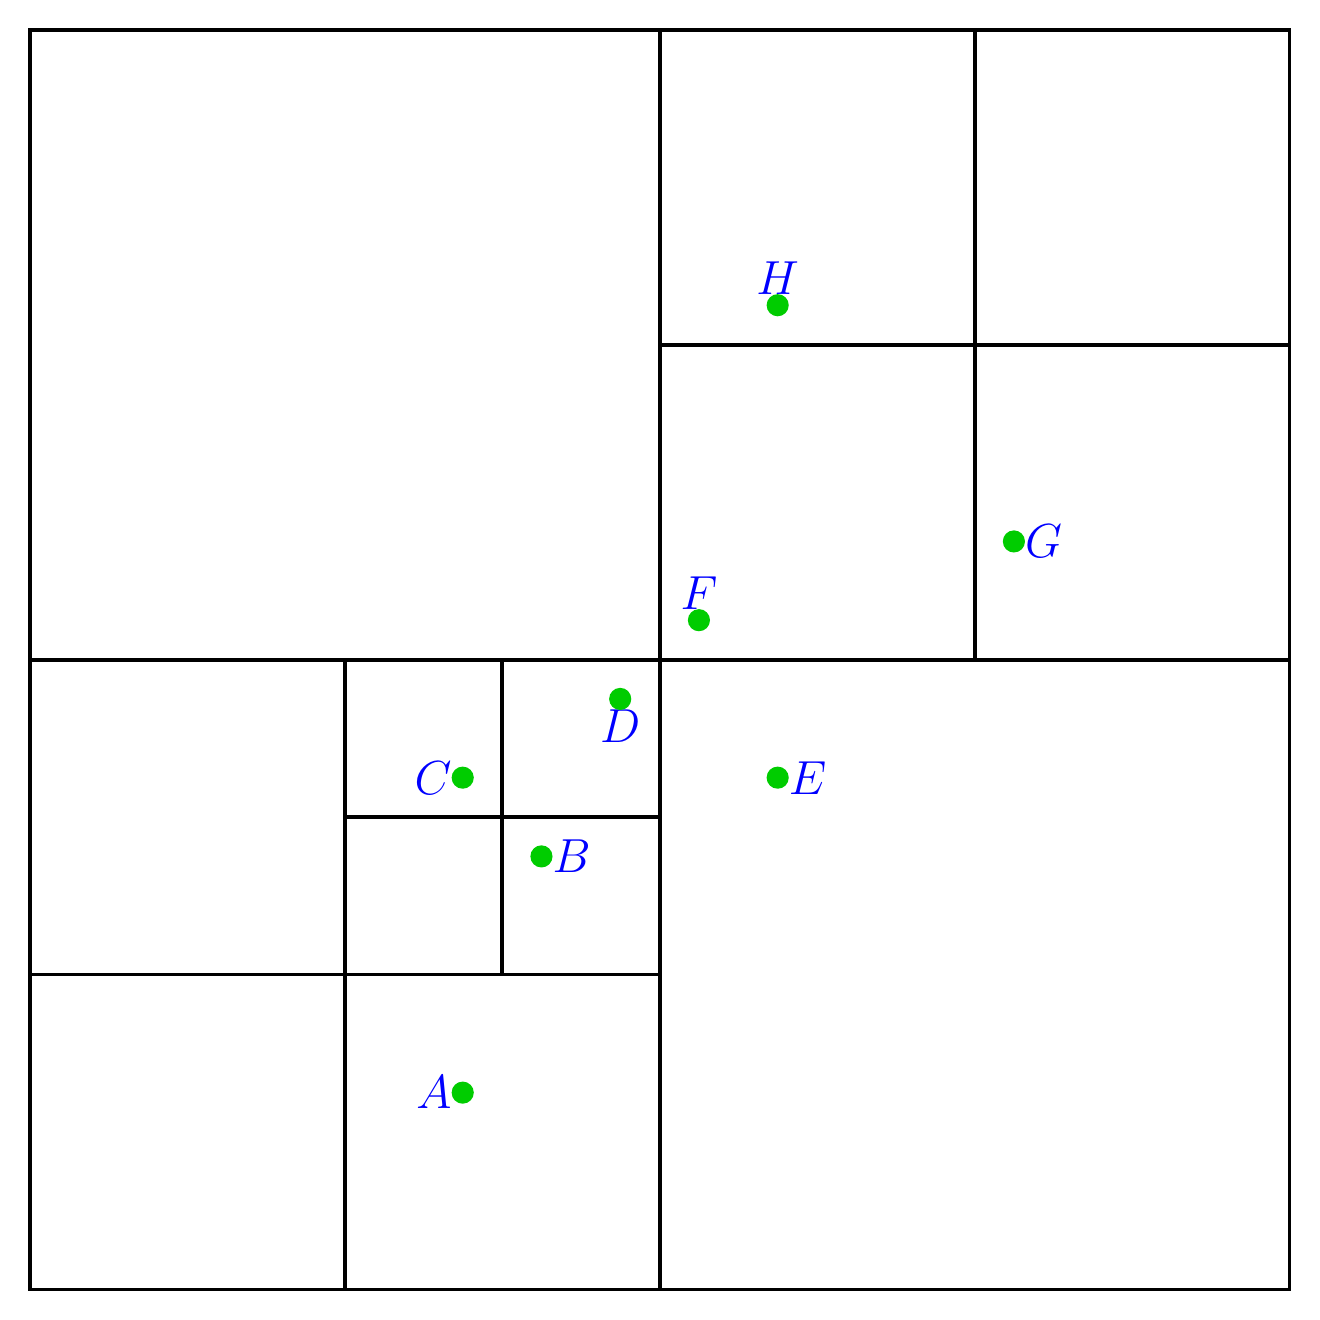
\begin{tikzpicture}[line width=.5mm]
    \def\A{\LARGE{\textcolor{blue}{$A$}}}
    \def\B{\LARGE{\textcolor{blue}{$B$}}}
    \def\C{\LARGE{\textcolor{blue}{$C$}}}
    \def\D{\LARGE{\textcolor{blue}{$D$}}}
    \def\E{\LARGE{\textcolor{blue}{$E$}}}
    \def\F{\LARGE{\textcolor{blue}{$F$}}}
    \def\G{\LARGE{\textcolor{blue}{$G$}}}
    \def\H{\LARGE{\textcolor{blue}{$H$}}}

    \draw (0, 0) rectangle (16, 16);

    \coordinate [label=left:\A] (A) at (5.5, 2.5);
    \coordinate [label=right:\B] (B) at (6.5, 5.5);
    \coordinate [label=left:\C] (C) at (5.5, 6.5);
    \coordinate [label=below:\D] (D) at (7.5, 7.5);
    \coordinate [label=right:\E] (E) at (9.5, 6.5);
    \coordinate [label=above:\F] (F) at (8.5, 8.5);
    \coordinate [label=right:\G] (G) at (12.5, 9.5);
    \coordinate [label=above:\H] (H) at (9.5, 12.5);

    \draw (8, 0) -- (8, 16);
    \draw (0, 8) -- (16, 8);
    \draw (4, 0) -- (4, 8);
    \draw (0, 4) -- (8, 4);
    \draw (4, 6) -- (8, 6);
    \draw (6, 4) -- (6, 8);
    \draw (8, 12) -- (16, 12);
    \draw (12, 8) -- (12, 16);

    \foreach \point in {A, B, C, D, E, F, G, H}
        \fill [green!80!black] (\point) circle (4pt);
\end{tikzpicture}

% vim: set ff=unix tw=79 sw=4 ts=4 et ic ai :

        }
        \caption{spatial partition}
    \end{figure}
\end{frame}

\subsection{Quadtree \& Morton Curve}
\begin{frame}
    \frametitle{Quadtree \& Morton Curve}
    \textbf{Properties:}
    \begin{itemize}
        \item The four children of a given a node are numbered consecutively
            $0,\dots,3$ \\
        \item When stepping through the levels of the tree towards a given
            point, the numbers of the nodes add up to the points morton key
            (possibly truncated) \\
        \item Points with a common parent node are neighbouring on the morton
            curve
    \end{itemize}
\end{frame}

\begin{frame}
    \begin{figure}
        \centering
        \caption{key = 0b001110}
        \resizebox{.6\textwidth}{!}{%
            \begin{tikzpicture} [tree layout, scale=\textwidth/10cm]
    \graph {%
        ROOT [rn] -- {[fresh nodes]%
            00 [query] -- {%
                01 [branch], 11 [query] -- {%
                    01 [branch], 10 [query], 11 [branch]
                }
            }, 01 [branch], 11 [branch] -- {%
                00 [branch], 01 [branch], 10 [branch]
            }
        }
    };
\end{tikzpicture}

        }
    \end{figure}

    \noindent\rule{\textwidth}{1pt}

    \textbf{Notes:}
    \begin{itemize}
        \item max depth of tree $=\frac{\textrm{key length}}{\textrm{dim}}$ \\
        \item Resolution of domain partitioned by the tree $=2^{\textrm{tree
            depth}}-1$
    \end{itemize}
\end{frame}

\begin{frame}
    \begin{figure}
        \centering
        \begin{animateinline}[controls={step,play,stop},buttonsize=10pt]{.5}
            \multiframe{4}{i=1+1}{%
                \resizebox{.7\textwidth}{!}{%
                    \begin{tikzpicture}[line width=.5mm, morton/.style={every
    path/.style={draw=gray, line width=.5mm}}]
    \drawpoints

    \ifthenelse{\i > 0}{%
        \draw (8, 0) -- (8, 16);
        \draw (0, 8) -- (16, 8);
    }{}

    \ifthenelse{\i = 1}{%
        \coordinate [label=45:\nodelabel{00}] (00) at (0, 0);
        \coordinate [label=45:\nodelabel{01}] (01) at (8, 0);
        \coordinate [label=315:\nodelabel{10}] (10) at (0, 16);
        \coordinate [label=315:\nodelabel{11}] (11) at (8, 16);
    }{}

    \ifthenelse{\i > 1}{%
        \draw (4, 0) -- (4, 8);
        \draw (0, 4) -- (8, 4);
        \draw (8, 12) -- (16, 12);
        \draw (12, 8) -- (12, 16);
    }{}

    \ifthenelse{\i = 2}{%
        \begin{pgfonlayer}{background}
            \fill[orange!20] (0,0) -- (8,0) -- (8,8) -- (0,8) -- cycle;
            \fill[orange!20] (8,8) -- (16,8) -- (16,16) -- (8,16) -- cycle;
        \end{pgfonlayer}
        \coordinate [label=45:\nodelabel{0000}] (0000) at (0, 0);
        \coordinate [label=45:\nodelabel{0001}] (0001) at (4, 0);
        \coordinate [label=45:\nodelabel{0010}] (0010) at (0, 4);
        \coordinate [label=45:\nodelabel{0011}] (0011) at (4, 4);
        \coordinate [label=315:\nodelabel{1100}] (1100) at (8, 12);
        \coordinate [label=315:\nodelabel{1101}] (1101) at (12, 12);
        \coordinate [label=315:\nodelabel{1110}] (1110) at (8, 16);
        \coordinate [label=315:\nodelabel{1111}] (1111) at (12, 16);
    }{}

    \ifthenelse{\i > 2}{%
        \draw (4, 6) -- (8, 6);
        \draw (6, 4) -- (6, 8);
    }{}

    \ifthenelse{\i = 3}{%
        \begin{pgfonlayer}{background}
            \fill[orange!20] (4,4) -- (8,4) -- (8,8) -- (4,8) -- cycle;
        \end{pgfonlayer}
        \coordinate [label=315:\nodelabel{001100}] (001100) at (4, 4);
        \coordinate [label=315:\nodelabel{001101}] (001101) at (6, 4);
        \coordinate [label=45:\nodelabel{001110}] (001110) at (4, 8);
        \coordinate [label=45:\nodelabel{001111}] (001111) at (6, 8);
    }{}

    \foreach \point in {A, B, C, D, E, F, G, H}
        \fill [black] (\point) circle (3pt);

    \ifthenelse{\i = 4}{%
        \begin{pgfonlayer}{background}
            \fill[orange!20] (4,6) -- (6,6) -- (6,8) -- (4,8) -- cycle;
        \end{pgfonlayer}

    \begin{scope}[morton]
        \draw (A) -- (B);
        \draw (B) -- (C);
        \draw (C) -- (D);
        \draw (D) -- (E);
        \draw (E) -- (F);
        \draw (F) -- (G);
        \draw (G) -- (H);
    \end{scope}

        \foreach \point in {A, B, C, D, E, F, G, H}
            \fill [black] (\point) circle (3pt);
        \coordinate [label=left:\nodelabel{(5,6)}] (mortonC) at (5.5, 6.5);
        \coordinate [label=45:\nodelabel{00111001}] (pointC) at (4, 8);
        \fill [red] (C) circle (3pt);
    }{}

\end{tikzpicture}

                }
            }
        \end{animateinline}
        \caption{Connection between keys of node and point}
    \end{figure}
\end{frame}

% vim: set ff=unix tw=79 sw=4 ts=4 et ic ai :

        }
    \end{figure}
\end{frame}

\begin{frame}
    \begin{figure}
        \centering
        \resizebox{.8\textwidth}{!}{%
            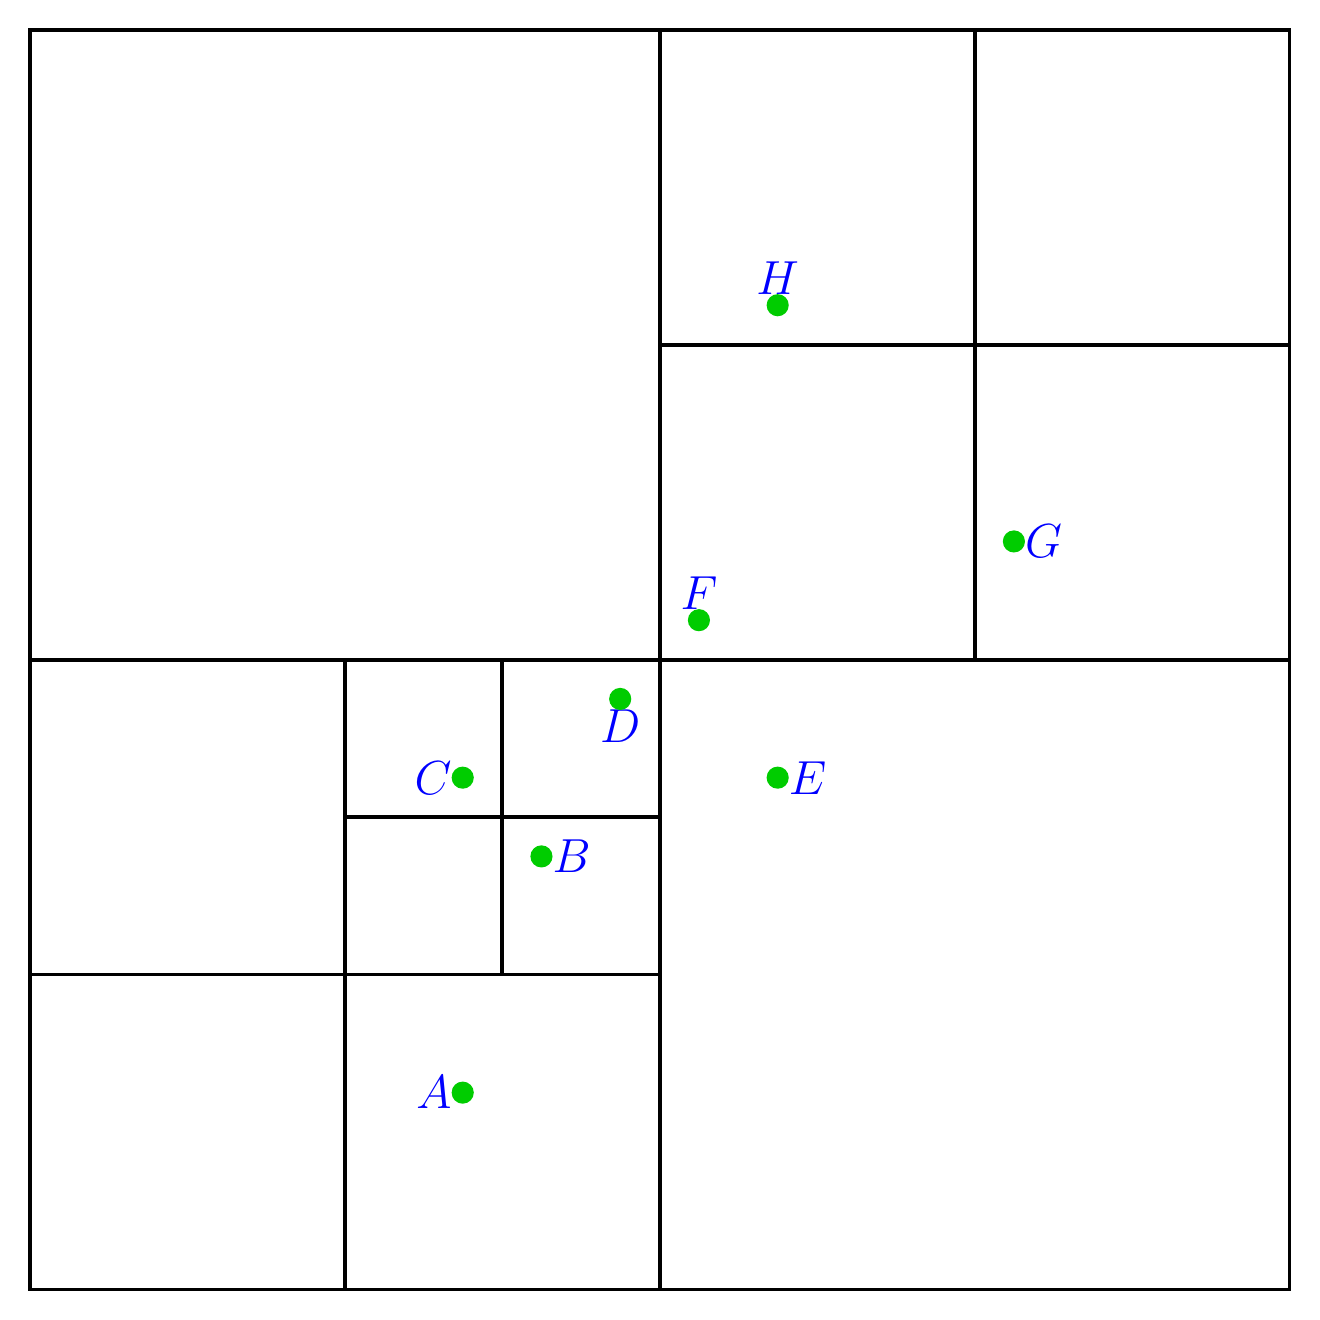
\begin{tikzpicture}[line width=.5mm]
    \def\A{\LARGE{\textcolor{blue}{$A$}}}
    \def\B{\LARGE{\textcolor{blue}{$B$}}}
    \def\C{\LARGE{\textcolor{blue}{$C$}}}
    \def\D{\LARGE{\textcolor{blue}{$D$}}}
    \def\E{\LARGE{\textcolor{blue}{$E$}}}
    \def\F{\LARGE{\textcolor{blue}{$F$}}}
    \def\G{\LARGE{\textcolor{blue}{$G$}}}
    \def\H{\LARGE{\textcolor{blue}{$H$}}}

    \draw (0, 0) rectangle (16, 16);

    \coordinate [label=left:\A] (A) at (5.5, 2.5);
    \coordinate [label=right:\B] (B) at (6.5, 5.5);
    \coordinate [label=left:\C] (C) at (5.5, 6.5);
    \coordinate [label=below:\D] (D) at (7.5, 7.5);
    \coordinate [label=right:\E] (E) at (9.5, 6.5);
    \coordinate [label=above:\F] (F) at (8.5, 8.5);
    \coordinate [label=right:\G] (G) at (12.5, 9.5);
    \coordinate [label=above:\H] (H) at (9.5, 12.5);

    \draw (8, 0) -- (8, 16);
    \draw (0, 8) -- (16, 8);
    \draw (4, 0) -- (4, 8);
    \draw (0, 4) -- (8, 4);
    \draw (4, 6) -- (8, 6);
    \draw (6, 4) -- (6, 8);
    \draw (8, 12) -- (16, 12);
    \draw (12, 8) -- (12, 16);

    \foreach \point in {A, B, C, D, E, F, G, H}
        \fill [green!80!black] (\point) circle (4pt);
\end{tikzpicture}

% vim: set ff=unix tw=79 sw=4 ts=4 et ic ai :

        }
        \caption{spatial partition}
    \end{figure}
\end{frame}

\subsection{Quadtree \& Morton Curve}
\begin{frame}
    \frametitle{Quadtree \& Morton Curve}
    \textbf{Properties:}
    \begin{itemize}
        \item The four children of a given a node are numbered consecutively
            $0,\dots,3$ \\
        \item When stepping through the levels of the tree towards a given
            point, the numbers of the nodes add up to the points morton key
            (possibly truncated) \\
        \item Points with a common parent node are neighbouring on the morton
            curve
    \end{itemize}
\end{frame}

\begin{frame}
    \begin{figure}
        \centering
        \caption{key = 0b001110}
        \resizebox{.6\textwidth}{!}{%
            \begin{tikzpicture} [tree layout, scale=\textwidth/10cm]
    \graph {%
        ROOT [rn] -- {[fresh nodes]%
            00 [query] -- {%
                01 [branch], 11 [query] -- {%
                    01 [branch], 10 [query], 11 [branch]
                }
            }, 01 [branch], 11 [branch] -- {%
                00 [branch], 01 [branch], 10 [branch]
            }
        }
    };
\end{tikzpicture}

        }
    \end{figure}

    \noindent\rule{\textwidth}{1pt}

    \textbf{Notes:}
    \begin{itemize}
        \item max depth of tree $=\frac{\textrm{key length}}{\textrm{dim}}$ \\
        \item Resolution of domain partitioned by the tree $=2^{\textrm{tree
            depth}}-1$
    \end{itemize}
\end{frame}

\begin{frame}
    \begin{figure}
        \centering
        \begin{animateinline}[controls={step,play,stop},buttonsize=10pt]{.5}
            \multiframe{4}{i=1+1}{%
                \resizebox{.7\textwidth}{!}{%
                    \begin{tikzpicture}[line width=.5mm, morton/.style={every
    path/.style={draw=gray, line width=.5mm}}]
    \drawpoints

    \ifthenelse{\i > 0}{%
        \draw (8, 0) -- (8, 16);
        \draw (0, 8) -- (16, 8);
    }{}

    \ifthenelse{\i = 1}{%
        \coordinate [label=45:\nodelabel{00}] (00) at (0, 0);
        \coordinate [label=45:\nodelabel{01}] (01) at (8, 0);
        \coordinate [label=315:\nodelabel{10}] (10) at (0, 16);
        \coordinate [label=315:\nodelabel{11}] (11) at (8, 16);
    }{}

    \ifthenelse{\i > 1}{%
        \draw (4, 0) -- (4, 8);
        \draw (0, 4) -- (8, 4);
        \draw (8, 12) -- (16, 12);
        \draw (12, 8) -- (12, 16);
    }{}

    \ifthenelse{\i = 2}{%
        \begin{pgfonlayer}{background}
            \fill[orange!20] (0,0) -- (8,0) -- (8,8) -- (0,8) -- cycle;
            \fill[orange!20] (8,8) -- (16,8) -- (16,16) -- (8,16) -- cycle;
        \end{pgfonlayer}
        \coordinate [label=45:\nodelabel{0000}] (0000) at (0, 0);
        \coordinate [label=45:\nodelabel{0001}] (0001) at (4, 0);
        \coordinate [label=45:\nodelabel{0010}] (0010) at (0, 4);
        \coordinate [label=45:\nodelabel{0011}] (0011) at (4, 4);
        \coordinate [label=315:\nodelabel{1100}] (1100) at (8, 12);
        \coordinate [label=315:\nodelabel{1101}] (1101) at (12, 12);
        \coordinate [label=315:\nodelabel{1110}] (1110) at (8, 16);
        \coordinate [label=315:\nodelabel{1111}] (1111) at (12, 16);
    }{}

    \ifthenelse{\i > 2}{%
        \draw (4, 6) -- (8, 6);
        \draw (6, 4) -- (6, 8);
    }{}

    \ifthenelse{\i = 3}{%
        \begin{pgfonlayer}{background}
            \fill[orange!20] (4,4) -- (8,4) -- (8,8) -- (4,8) -- cycle;
        \end{pgfonlayer}
        \coordinate [label=315:\nodelabel{001100}] (001100) at (4, 4);
        \coordinate [label=315:\nodelabel{001101}] (001101) at (6, 4);
        \coordinate [label=45:\nodelabel{001110}] (001110) at (4, 8);
        \coordinate [label=45:\nodelabel{001111}] (001111) at (6, 8);
    }{}

    \foreach \point in {A, B, C, D, E, F, G, H}
        \fill [black] (\point) circle (3pt);

    \ifthenelse{\i = 4}{%
        \begin{pgfonlayer}{background}
            \fill[orange!20] (4,6) -- (6,6) -- (6,8) -- (4,8) -- cycle;
        \end{pgfonlayer}

    \begin{scope}[morton]
        \draw (A) -- (B);
        \draw (B) -- (C);
        \draw (C) -- (D);
        \draw (D) -- (E);
        \draw (E) -- (F);
        \draw (F) -- (G);
        \draw (G) -- (H);
    \end{scope}

        \foreach \point in {A, B, C, D, E, F, G, H}
            \fill [black] (\point) circle (3pt);
        \coordinate [label=left:\nodelabel{(5,6)}] (mortonC) at (5.5, 6.5);
        \coordinate [label=45:\nodelabel{00111001}] (pointC) at (4, 8);
        \fill [red] (C) circle (3pt);
    }{}

\end{tikzpicture}

                }
            }
        \end{animateinline}
        \caption{Connection between keys of node and point}
    \end{figure}
\end{frame}

% vim: set ff=unix tw=79 sw=4 ts=4 et ic ai :

        }
    \end{figure}
\end{frame}

\begin{frame}
    \begin{figure}
        \centering
        \resizebox{.8\textwidth}{!}{%
            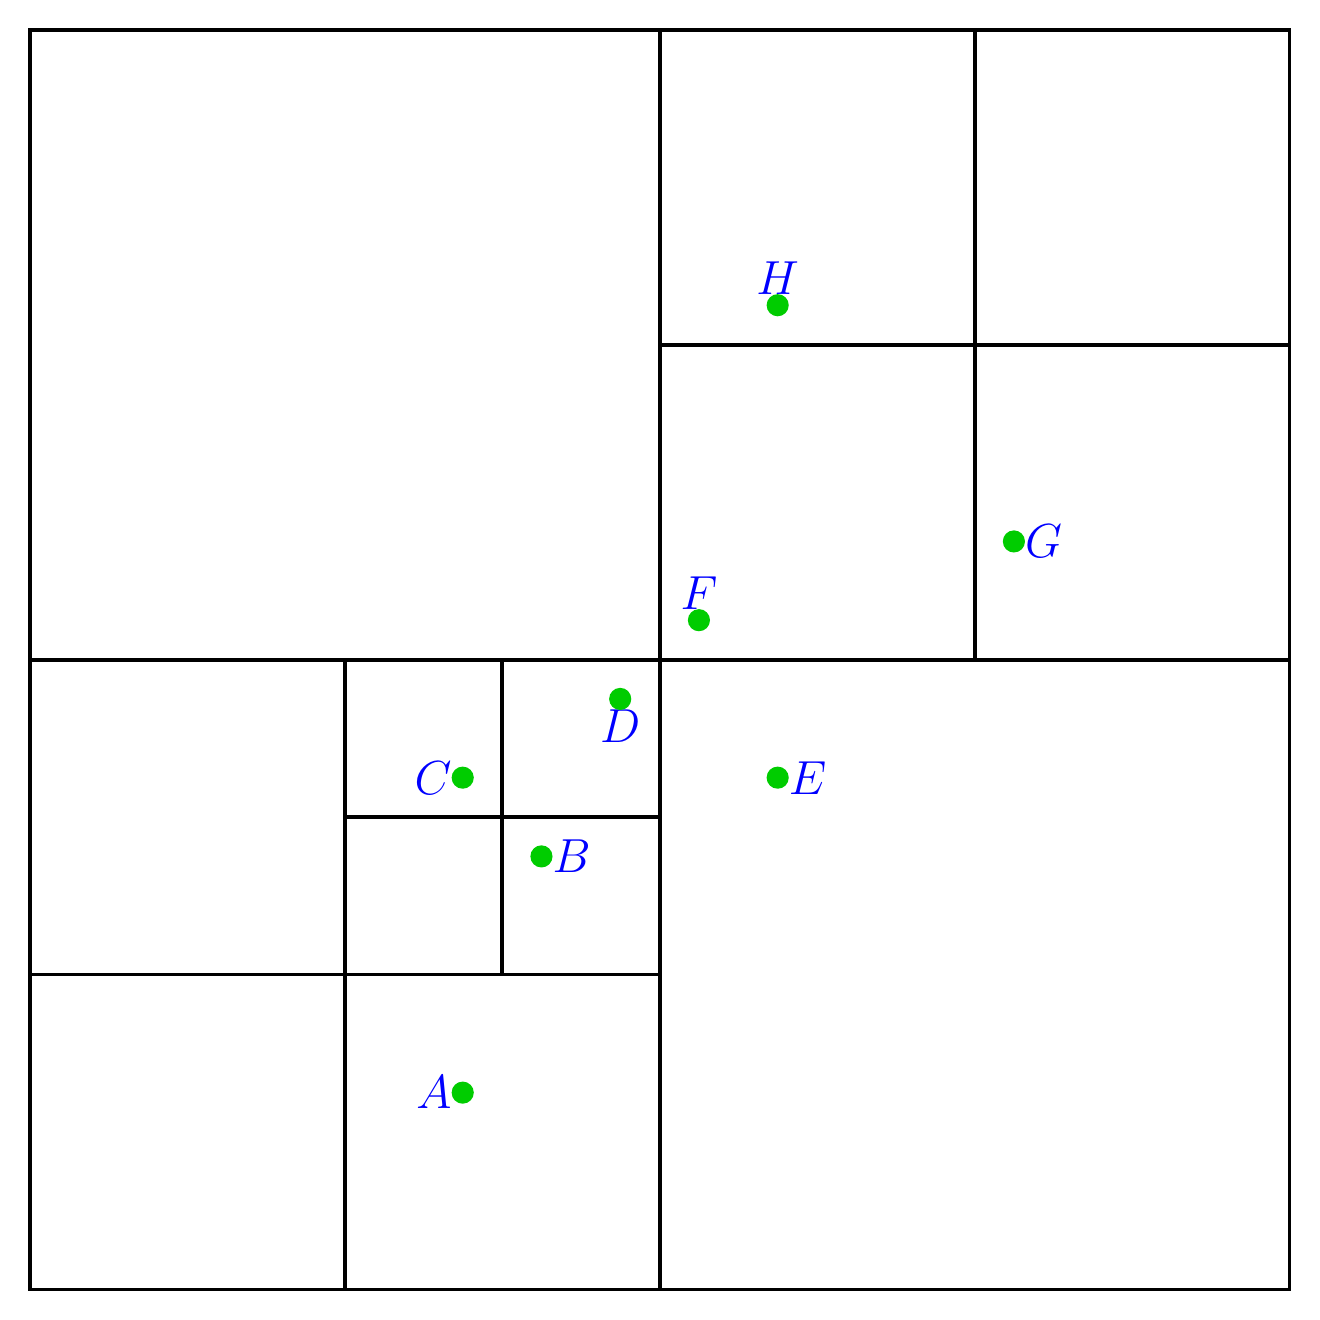
\begin{tikzpicture}[line width=.5mm]
    \def\A{\LARGE{\textcolor{blue}{$A$}}}
    \def\B{\LARGE{\textcolor{blue}{$B$}}}
    \def\C{\LARGE{\textcolor{blue}{$C$}}}
    \def\D{\LARGE{\textcolor{blue}{$D$}}}
    \def\E{\LARGE{\textcolor{blue}{$E$}}}
    \def\F{\LARGE{\textcolor{blue}{$F$}}}
    \def\G{\LARGE{\textcolor{blue}{$G$}}}
    \def\H{\LARGE{\textcolor{blue}{$H$}}}

    \draw (0, 0) rectangle (16, 16);

    \coordinate [label=left:\A] (A) at (5.5, 2.5);
    \coordinate [label=right:\B] (B) at (6.5, 5.5);
    \coordinate [label=left:\C] (C) at (5.5, 6.5);
    \coordinate [label=below:\D] (D) at (7.5, 7.5);
    \coordinate [label=right:\E] (E) at (9.5, 6.5);
    \coordinate [label=above:\F] (F) at (8.5, 8.5);
    \coordinate [label=right:\G] (G) at (12.5, 9.5);
    \coordinate [label=above:\H] (H) at (9.5, 12.5);

    \draw (8, 0) -- (8, 16);
    \draw (0, 8) -- (16, 8);
    \draw (4, 0) -- (4, 8);
    \draw (0, 4) -- (8, 4);
    \draw (4, 6) -- (8, 6);
    \draw (6, 4) -- (6, 8);
    \draw (8, 12) -- (16, 12);
    \draw (12, 8) -- (12, 16);

    \foreach \point in {A, B, C, D, E, F, G, H}
        \fill [green!80!black] (\point) circle (4pt);
\end{tikzpicture}

% vim: set ff=unix tw=79 sw=4 ts=4 et ic ai :

        }
        \caption{spatial partition}
    \end{figure}
\end{frame}

\subsection{Quadtree \& Morton Curve}
\begin{frame}
    \frametitle{Quadtree \& Morton Curve}
    \textbf{Properties:}
    \begin{itemize}
        \item The four children of a given a node are numbered consecutively
            $0,\dots,3$ \\
        \item When stepping through the levels of the tree towards a given
            point, the numbers of the nodes add up to the points morton key
            (possibly truncated) \\
        \item Points with a common parent node are neighbouring on the morton
            curve
    \end{itemize}
\end{frame}

\begin{frame}
    \begin{figure}
        \centering
        \caption{key = 0b001110}
        \resizebox{.6\textwidth}{!}{%
            \begin{tikzpicture} [tree layout, scale=\textwidth/10cm]
    \graph {%
        ROOT [rn] -- {[fresh nodes]%
            00 [query] -- {%
                01 [branch], 11 [query] -- {%
                    01 [branch], 10 [query], 11 [branch]
                }
            }, 01 [branch], 11 [branch] -- {%
                00 [branch], 01 [branch], 10 [branch]
            }
        }
    };
\end{tikzpicture}

        }
    \end{figure}

    \noindent\rule{\textwidth}{1pt}

    \textbf{Notes:}
    \begin{itemize}
        \item max depth of tree $=\frac{\textrm{key length}}{\textrm{dim}}$ \\
        \item Resolution of domain partitioned by the tree $=2^{\textrm{tree
            depth}}-1$
    \end{itemize}
\end{frame}

\begin{frame}
    \begin{figure}
        \centering
        \begin{animateinline}[controls={step,play,stop},buttonsize=10pt]{.5}
            \multiframe{4}{i=1+1}{%
                \resizebox{.7\textwidth}{!}{%
                    \begin{tikzpicture}[line width=.5mm, morton/.style={every
    path/.style={draw=gray, line width=.5mm}}]
    \drawpoints

    \ifthenelse{\i > 0}{%
        \draw (8, 0) -- (8, 16);
        \draw (0, 8) -- (16, 8);
    }{}

    \ifthenelse{\i = 1}{%
        \coordinate [label=45:\nodelabel{00}] (00) at (0, 0);
        \coordinate [label=45:\nodelabel{01}] (01) at (8, 0);
        \coordinate [label=315:\nodelabel{10}] (10) at (0, 16);
        \coordinate [label=315:\nodelabel{11}] (11) at (8, 16);
    }{}

    \ifthenelse{\i > 1}{%
        \draw (4, 0) -- (4, 8);
        \draw (0, 4) -- (8, 4);
        \draw (8, 12) -- (16, 12);
        \draw (12, 8) -- (12, 16);
    }{}

    \ifthenelse{\i = 2}{%
        \begin{pgfonlayer}{background}
            \fill[orange!20] (0,0) -- (8,0) -- (8,8) -- (0,8) -- cycle;
            \fill[orange!20] (8,8) -- (16,8) -- (16,16) -- (8,16) -- cycle;
        \end{pgfonlayer}
        \coordinate [label=45:\nodelabel{0000}] (0000) at (0, 0);
        \coordinate [label=45:\nodelabel{0001}] (0001) at (4, 0);
        \coordinate [label=45:\nodelabel{0010}] (0010) at (0, 4);
        \coordinate [label=45:\nodelabel{0011}] (0011) at (4, 4);
        \coordinate [label=315:\nodelabel{1100}] (1100) at (8, 12);
        \coordinate [label=315:\nodelabel{1101}] (1101) at (12, 12);
        \coordinate [label=315:\nodelabel{1110}] (1110) at (8, 16);
        \coordinate [label=315:\nodelabel{1111}] (1111) at (12, 16);
    }{}

    \ifthenelse{\i > 2}{%
        \draw (4, 6) -- (8, 6);
        \draw (6, 4) -- (6, 8);
    }{}

    \ifthenelse{\i = 3}{%
        \begin{pgfonlayer}{background}
            \fill[orange!20] (4,4) -- (8,4) -- (8,8) -- (4,8) -- cycle;
        \end{pgfonlayer}
        \coordinate [label=315:\nodelabel{001100}] (001100) at (4, 4);
        \coordinate [label=315:\nodelabel{001101}] (001101) at (6, 4);
        \coordinate [label=45:\nodelabel{001110}] (001110) at (4, 8);
        \coordinate [label=45:\nodelabel{001111}] (001111) at (6, 8);
    }{}

    \foreach \point in {A, B, C, D, E, F, G, H}
        \fill [black] (\point) circle (3pt);

    \ifthenelse{\i = 4}{%
        \begin{pgfonlayer}{background}
            \fill[orange!20] (4,6) -- (6,6) -- (6,8) -- (4,8) -- cycle;
        \end{pgfonlayer}

    \begin{scope}[morton]
        \draw (A) -- (B);
        \draw (B) -- (C);
        \draw (C) -- (D);
        \draw (D) -- (E);
        \draw (E) -- (F);
        \draw (F) -- (G);
        \draw (G) -- (H);
    \end{scope}

        \foreach \point in {A, B, C, D, E, F, G, H}
            \fill [black] (\point) circle (3pt);
        \coordinate [label=left:\nodelabel{(5,6)}] (mortonC) at (5.5, 6.5);
        \coordinate [label=45:\nodelabel{00111001}] (pointC) at (4, 8);
        \fill [red] (C) circle (3pt);
    }{}

\end{tikzpicture}

                }
            }
        \end{animateinline}
        \caption{Connection between keys of node and point}
    \end{figure}
\end{frame}

\subsection{Example}
\begin{frame}
    \textbf{Space Seperation Animation}
    \begin{center}
        \animategraphics[%
            % draft,
            % every=3,
            type=png,
            width=.99 \textwidth,
            controls={play,step,stop},
            buttonsize=10pt
        ]{3}{plots/out-}{000}{064}
    \end{center}
\end{frame}


\begin{frame}
    \textbf{Quadtree Construction}
    \begin{center}
        \animategraphics[%
            % draft,
            % every=3,
            type=png,
            width=\textwidth,
            controls={play,step,stop},
            buttonsize=10pt
        ]{3}{graphs/extent_out-}{001}{063}
    \end{center}
\end{frame}

% vim: set ff=unix tw=79 sw=4 ts=4 et ic ai :
